\documentclass[a4paper,12pt]{report}

\usepackage[utf8]{inputenc}
\usepackage[french]{babel}
\usepackage[T1]{fontenc}
\usepackage[scaled]{helvet} % police
\usepackage{lmodern}
\usepackage{layout}
\usepackage[top=2cm, bottom=2cm, left=3cm, right=2cm]{geometry}
\usepackage{setspace}
\usepackage{verbatim}
\usepackage{moreverb}
\usepackage{listings}
\usepackage{graphicx}
\usepackage{shorttoc}
\usepackage{glossaries}
\usepackage{xcolor}
\usepackage{eurosym}
\usepackage{amsmath}

\usepackage{xcolor}
%\usepackage{biblatex} 

% Tête de chapitre
\makeatletter
\newlength{\chapter@number@width}
\def\@makechapterhead#1{%
  {\normalfont
  \setlength{\parindent}{0pt}%
  \vspace*{10pt}%
  \settowidth{\chapter@number@width}{%
    \hbox{\color{white}\LARGE\bfseries
          \hspace{\dimexpr 1mm+3pt}%
          \thechapter
          \hspace{\dimexpr 1mm+3pt}%
    }}
  \hbox{%
    \vtop{%
      \hsize=\dimexpr\chapter@number@width+\tabcolsep+2\fboxrule+\tabcolsep
      \begin{tabular}[t]{@{}c}
        \scshape\strut\makebox[0pt]{\hspace{0pt plus 1 fill minus 1 fill}\@chapapp\hspace{0pt plus 1 fill minus 1 fill}} \\
        \fboxsep=0pt
        \colorbox{black}{\vbox{%
           \hbox{\vbox to \dimexpr 1mm+3pt{}}
           \hbox{\color{white}\LARGE\bfseries
                 \hspace{\dimexpr 1mm+3pt}%
                 \thechapter
                 \hspace{\dimexpr 1mm+3pt}%
                }
           \hrule height 0.4pt depth 0pt width 0pt
           \hbox{\vbox to 6pt{}}
           \hbox{\parbox{0pt}{\Huge\bfseries\vphantom{E}}}
           }}%
      \end{tabular}%
      }%
    \vtop{%
      \advance\hsize by -\dimexpr\chapter@number@width+2\fboxrule+\tabcolsep
      \hspace*{-0.5cm}\begin{tabular}[t]{c}
        \scshape\strut\vphantom{\@chapapp} \\
        \fboxsep=0pt
        \colorbox{white}{\vbox{%
           \hbox{\vbox to \dimexpr 1mm+3pt{}}
           \hbox{\LARGE\bfseries
                 \hspace{\dimexpr 1mm+3pt}%
                 \phantom{\thechapter}
                 \hspace{\dimexpr 1mm+3pt}%
                }
           \hrule height 0.4pt depth 0pt width \hsize
           \hbox{\vbox to 6pt{}}
           \hbox{\hspace*{20pt}\parbox{\dimexpr\textwidth-2mm-6pt-\chapter@number@width-\tabcolsep-2\fboxrule-20pt}{\Huge\bfseries #1}}
           }}%
      \end{tabular}%
      }%
    }%
  \vspace{50pt}%
  }
}
\def\@makeschapterhead#1{%
  {\normalfont
  \setlength{\parindent}{0pt}%
  \vspace*{10pt}%
  \settowidth{\chapter@number@width}{%
    \hbox{\color{white}\LARGE\bfseries
          \hspace{\dimexpr 1mm+3pt}%
          \thechapter
          \hspace{\dimexpr 1mm+3pt}%
    }}
  \hbox{%
    \vtop{%
      \hsize=\dimexpr\chapter@number@width+\tabcolsep+2\fboxrule+\tabcolsep
      \begin{tabular}[t]{@{}c}
        \scshape\strut\makebox[0pt]{\hspace{0pt plus 1 fill minus 1 fill}\phantom{\@chapapp}\hspace{0pt plus 1 fill minus 1 fill}} \\
        \fboxsep=0pt
        \colorbox{black}{\vbox{%
           \hbox{\vbox to \dimexpr 1mm+3pt{}}
           \hbox{\color{white}\LARGE\bfseries
                 \hspace{\dimexpr 1mm+3pt}%
                 \phantom{\thechapter}%
                 \hspace{\dimexpr 1mm+3pt}%
                }
           \hrule height 0.4pt depth 0pt width 0pt
           \hbox{\vbox to 6pt{}}
           \hbox{\parbox{0pt}{\Huge\bfseries\vphantom{E}}}
           }}%
      \end{tabular}%
      }%
    \vtop{%
      \advance\hsize by -\dimexpr\chapter@number@width+2\fboxrule+\tabcolsep
      \hspace*{-0.5cm}\begin{tabular}[t]{c}
        \scshape\strut\vphantom{\@chapapp} \\
        \fboxsep=0pt
        \colorbox{white}{\vbox{%
           \hbox{\vbox to \dimexpr 1mm+3pt{}}
           \hbox{\LARGE\bfseries
                 \hspace{\dimexpr 1mm+3pt}%
                 \phantom{\thechapter}
                 \hspace{\dimexpr 1mm+3pt}%
                }
           \hrule height 0.4pt depth 0pt width \hsize
           \hbox{\vbox to 6pt{}}
           \hbox{\hspace*{20pt}\parbox{\dimexpr\textwidth-2mm-6pt-\chapter@number@width-\tabcolsep-2\fboxrule-20pt}{\Huge\bfseries #1}}
           }}%
      \end{tabular}%
      }%
    }%
  \vspace{50pt}%
  }
}
\makeatother

% Redéfinition de commandes
\renewcommand\thesection{\arabic{section}}
% \renewcommand\thechapter{\Roman{chapter}}
\renewcommand*\familydefault{\sfdefault} %% Only if the base font of the document is to be sans serif

\makeglossaries
\newglossaryentry{ASP}{
	name={ASP}, % apparait dans le glossaire
	text={ASP*}, % apparait dans le texte
	description={Application Service Provider,  Fournisseur d'Applications de Service}
}
\newglossaryentry{CMS}{
	name={CMS}, % apparait dans le glossaire
	text={CMS*}, % apparait dans le texte
	description={(Content Management System ou système de gestion de contenu) : logiciel destiné à la conception et à la mise à jour dynamique de site Web ou d’application multimédia.}
} 
\newglossaryentry{CRM}{
	name={CRM},
	text={CRM*},
	description={(Customer Relationship Management ou gestion de la relation client) : ensemble des outils et techniques destinés à capter, traiter, analyser les informations relatives aux clients et aux prospects, dans le but de les fidéliser en leur offrant le meilleur service.}
}

\title{Le cloud et la virtualisation}
\author{Sébastien Corbin et Gaëlle Avrillon}
\date{\today}


\begin{document}
% Interlignage 1,5
\begin{onehalfspace}

		\begin{titlepage}
			\begin{center}
				Sébastien CORBIN et Gaëlle AVRILLON\\
				CSII 3\ieme année\\
			\end{center}
			\hrulefill
			\vspace{7cm}
			\begin{center} 
				\LARGE \textbf{La virtualisation et le cloud}\\
			\end{center}
		\end{titlepage}
		\newpage

		\shorttableofcontents{Sommaire}{1}
		\setcounter{page}{1}
		\thispagestyle{empty}
		\newpage

	%%%%%%%%%%%%%%%%%%
	% Introduction 
	%%%%%%%%%%%%%%%%%%
	\chapter*{Introduction}
	
	\paragraph*{}
	Le Cloud Computing est un concept qui consiste à déporter sur des serveurs distants des traitements informatiques (applications, données) traditionnellement localisés sur des serveurs locaux ou encore sur le poste client de l’utilisateur. En français, l’anglicisme “Cloud Computing” est largement utilisé. Cependant, on rencontre de nombreuses traductions telles que “informatique dans le nuage”, “informatique dématérialisée”, “informatique virtuelle”, ou encore “infonuagique”.

	\paragraph*{}
	Les utilisateurs ou les entreprises ne gèrent plus leurs serveurs informatiques mais peuvent accéder de manière évolutive à de nombreux services en ligne. Les applications et les données ne sont plus présentes sur l’ordinateur local mais dans le nuage (“Cloud”). Le Cloud est composé d’un certain nombre de serveurs interconnectés. L’accès à ces services s’effectue la plupart du temps à l’aide d’un navigateur web.
	
	\paragraph*{}
	Le concept d'informatique dans le nuage est comparable à celui de la distribution de l'énergie électrique. La puissance de calcul et de stockage de l'information est proposée à la consommation par des entreprises spécialisées et facturée d'après l'utilisation réelle. Ainsi, les entreprises n'ont plus besoin de serveurs dédiés, mais confient cette ressource à une entreprise qui leur garantit une puissance de calcul et de stockage à la demande.
	
	\paragraph*{}
	Le Cloud a émergé pour répondre aux exigences de continuité de qualité de service. Il exprime la mise en flexibilité de 4 niveaux : l’application (en contact avec le client), la plateforme (qui exécute les applications), l’infrastructure (qui est le support de la plateforme) et les données (qui sont fournies sur demande).
	
	\paragraph*{}
%TODO Source HyperCloudMarket
	Plus de 100 milliards d’euros (selon CloudHyperMarket) ont été investi dans le cloud computing. Les deux principaux acteurs du Cloud Computing sont Microsoft et Google. Microsoft a investi 9,6 milliards de dollar en 2011 dans le cloud soit 90\% de ses dépenses en recherche et développement. 4 millions d’entreprises ont fait confiance à Google et sont passées à Google Apps. Elles profitent à présent de grandes améliorations en termes de collaboration et d'économies.
	
	\paragraph*{}
	On trouve les premières traces du “cloud computing” dans les années 1960, quand Johan McCarty affirmait que cette puissance de traitement informatique serait accessible au public dans le futur. On parlait alors de Bureaux de Services (Service bureaus). C’est l’ancêtre du Software as a Service. Leur point commun est qu’ils offrent un service en échange d’honoraires. Leur application dans les domaines est vaste : banques, assurances, etc. Une entreprise de ce type offre à ses clients son expertise dans un domaine : cela correspond tout à fait avec la notion actuelle de Software As A Service (SaaS) et c’est par l’avancée technologique des réseaux de communications que cette notion de “bureaux de service”  s’est énormément développée dans l’informatique.
	
	\paragraph*{}
	Cependant, les débuts du cloud computing se situent dans la notion de Fournisseur de Service d’Application (ou en anglais Application Service Provider, ASP), présente au début des années 2000. Les premières applications à avoir migré dans le nuage sont les messageries, les outils collaboratifs, le CRM*, les environnements de développement. Amazon, Yahoo et Google sont les premiers à se lancer dans ce concept. Ces deux derniers offrent au grand public des applications simples et gratuites telles que la messagerie ou la gestion de calendriers en ligne.
%TODO Glossaire CRM
	
	\paragraph*{}
	Le Grid Computing est une infrastructure virtuelle constituée d’un ensemble de ressources informatiques. Ces ressources sont partagées (elles sont mises à disposition des consommateurs), distribuées (elles sont situées dans des lieux géographiques différents), hétérogènes, coordonnées, autonomes et délocalisées (les ressources peuvent appartenir à plusieurs sites). On parle de “fermes de serveurs” (\textit{computer cluster} en anglais) pour désigner cette technique qui consiste à regrouper plusieurs ordinateurs / serveurs indépendants. Cette technique permet une gestion globale, augmente la disponibilité des ressources, facilite la montée en charge et permet une répartition des charges entre les différents serveurs.
	Une des premières entreprises à avoir utilisé cette technique est Google, celui-ci a du créer des fermes de serveurs spécialisées pour répondre au nombre gigantesque de requêtes devant être traitées chaque seconde.
	
	\paragraph*{}
	Le terme Software as a Service (abrégé SaaS) est apparu en 2007 et remplace les précédents termes tels que ASP (Application Service Provider) ou encore “On Demand”.
	C’est un concept consistant à proposer un abonnement au logiciel plutôt que l’achat d’une licence. Avec le développement des technologies de l’information, de nombreuses offres SaaS se font à travers le web. Il n’y a alors plus besoin d’installer d’application de bureau, qui est remplacée par un programme client-serveur.
	Les applications s’appuyant sur ce modèle ont été nativement conçues pour le web contrairement aux modèles précédents.
	
	\paragraph*{}
	La crise de 2008-2009 a fait de gros dégâts dans la plupart des secteurs d’activités. La principale préoccupation des gérants d’entreprise est d’économiser afin de limiter les effets de la crise sur leur structure. Le service informatique est un service qui coûte cher. En effet, il faut prendre en compte les salaires, les assurances, les locaux, le matériel informatique, ... Ces dépenses peuvent être réduites voire totalement éliminées grâce au cloud computing. Le cloud computing permet de s'affranchir des coûts d'installation et de maintenance du matériel informatique et des logiciels en interne, on peut également s'affranchir des employés effectuant cette tâche, et par conséquent de leur salaire, de leur matériel et de leurs locaux. Une économie non négligeable à l'échelle d'une petite comme d'une grande entreprise.

	Mais les gains en termes de coût ne sont pas la seule raison qui peuvent pousser les entreprises à choisir le cloud computing. Devant les besoins d'évolutivité et de flexibilité des grands acteurs de l'informatique, les notions comme le Grid Computing ou la virtualisation sont devenues incontournables.
	
	% TODO : faire un renvoi vers le grid computing
	
	\paragraph*{}
	Nous étudierons dans ce rapport \textbf{l’apport des technologies du Cloud dans les entreprises}.
	
	\paragraph*{}
	En effet, le Grid Computing trouve ses bases dans la virtualisation (voir ci-dessus), celle-ci étant  le fondement même du Cloud. Elle permet entre autres de faire fonctionner plusieurs systèmes d’exploitation sur un serveur physique au lieu d’en installer un par machine physique. Un autre objectif de la virtualisation est de pouvoir tester des applications sur des serveurs virtuels au lieu de serveurs physiques sans risques.
	
	Ces serveurs peuvent être hébergés au sein d’une entreprise ou chez un fournisseur de Cloud. Ainsi, on distingue trois architectures du Cloud : les clouds privés, les clouds publiques et les clouds hybrides. Le cloud privé est géré en interne par une entreprise pour ses propres besoins. Le cloud publique est géré par des entreprises spécialisées (les fournisseurs de services). Ces fournisseurs vont louer des ressources et des services à des entreprises ou à des particuliers. Enfin, le cloud hybride correspond à l’utilisation de plusieurs clouds (privés ou publiques).
	
	\paragraph*{}
	Dans un premier temps, nous présenterons le Cloud Computing. Puis, nous nous placerons dans un contexte d’entreprise afin d’étudier les besoins en terme de sécurité, de rentabilité et de flexibilité. Nous détaillerons ensuite les solutions techniques : les différentes architectures, la virtualisation. Nous finirons par un cas pratique en entreprise.
	
	
	
	%%%%%%%%%%%%%%%%%%%%%%%%%%
	\chapter{Présentation du Cloud Computing}
	%%%%%%%%%%%%%%%%%%%%%%%%%%


	%%%%%%%%%%%%%%%%%%%%%%%%%%
	\section{Définition du Cloud Computing}
	
	Le “Cloud Computing” est un néologisme utilisé pour décrire l’association d’Internet (“cloud”, le nuage) et l’utilisation de l’informatique (“computing”). On utilise l’informatique de manière dynamique et évolutive. Toutes les ressources sont fournies sous la forme de services à travers Internet. Les utilisateurs n’ont besoin d’aucune connaissance technique des services proposés.

	\paragraph*{}
	Ce concept inclut les infrastructures en tant que service (Infrastructure as a Service ou IaaS), les plateformes en tant que service (Platform as a Service ou PaaS), les applications en tant que service (Software as a Service ou SaaS) ainsi que le “Web 2.0” (aspect social d’Internet) et toutes les technologies récentes. Ces technologies dépendent presque exclusivement d’Internet pour répondre aux besoins des utilisateurs. Des exemples de fournisseurs de SaaS sont Salesforce.com ou encore Google Apps. Ils fournissent des outils professionnels accessibles par un navigateur web. Les applicatifs et les données sont stockés sur des serveurs distants.
	
	\paragraph*{}
	Le “cloud computing” correspond donc au développement et à l’utilisation d’applications accessibles uniquement par Internet. L’utilisateur a juste besoin d’Internet pour utiliser les applications, il n’a pas besoin d’installer un quelconque logiciel sur son poste. Les informations sont stockées de façon permanente sur Internet.
	
	\paragraph*{}
	La démocratisation des connexions Internet “haut débit” ainsi que l'accroissement de la capacité et de la puissance des disques durs et des processeurs ont permis le développement du “cloud computing”. Les utilisateurs louent du matériel auprès de leurs fournisseurs de service qui peuvent servir des millions de clients avec seulement des centaines de serveurs.
	
	\paragraph*{}
	Le cloud computing est perçu aujourd'hui comme quelque chose d'extrêmement puissant, capable de résoudre plusieurs milliards de milliards (10$^{18}$) de traitements informatiques à la seconde, ce qui est largement supérieur à n'importe lequel des ordinateurs de bureau modernes seulement capables de milliers de milliards (10$^{12}$) d'opérations à la seconde.
	
	\paragraph*{}
	Cette puissance est fournie par des architectures distribuées constituées d'ordinateurs « low-cost » (peu coûteux) qui s'échangent et se distribuent le travail en permanence. Elle est désormais à disposition de n'importe qui au travers d'Internet, que ce soit pour des utilisations financières (analyses), scientifiques (climat, statistiques) ou même médicales.
	

	%%%%%%%%%%%%%%%%%%%%%%%%%%
	\section{Les briques du Cloud Computing}

	Le cloud computing est une évolution naturelle des concepts de virtualisation, d’architecture basée sur les services (SaaS), et d’Utility Computing. Les utilisateurs n’ont plus besoin de détenir l’expertise du domaine informatique, ils louent la totalité de leur système d’information.
	
	\begin{figure}[!h]
		\centering
		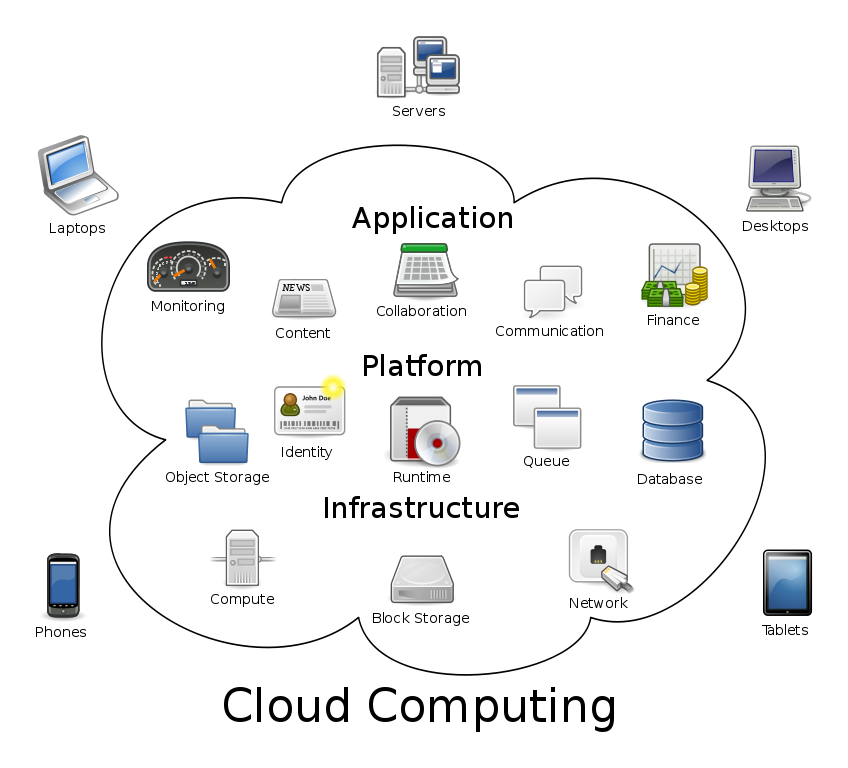
\includegraphics[width=15cm]{schema_structure.png}
		\caption{Le schéma du cloud computing}
	\end{figure}
	
	On distingue ainsi 3 briques principales dans le Cloud :
	\begin{itemize}
		\item Application (Software as a service, SaaS)
		\item Platform (Platform as a service, PaaS)
		\item Infrastructure (Infrastructure as service, IaaS)
	\end{itemize}
	
	\subsection{Application (SaaS)}
	L’acronyme “SaaS” est le plus connu dans le monde du cloud computing. Sa signification est “Software as a Service”, autrement dit “application en tant que service”.
	
	Les différents services loués par le fournisseur sont disponibles sur le web, accessibles via un navigateur et vont de la messagerie à l’ERP en passant par des outils collaboratifs (documents, agenda, etc.) ou la comptabilité en ligne. Cette méthode supprime la nécessité d’installer une application sur le poste client et permet de diminuer les coûts du parc informatique interne à l’entreprise cliente, simplifiant par la même le support et la maintenance du service.
	
	\paragraph*{}
	\underline{Exemples :}
	\begin{itemize}
		\item CRM Salesforce.com (http://www.salesforce.com)
		\item Google Docs (http://docs.google.com)
		\item Adobe Photoshop Express Online (http://www.photoshop.com/express)
	\end{itemize}

	\subsection{Plateforme (PaaS)}
	Le “PaaS” (“Platform as a Service” ou encore plate-forme en tant que service) a pour rôle l’exécution du logiciel. Elle est composée de briques utilisant des langages de programmation de haut niveau, généralement des langages de script (console de commande, Python, SQL, serveur d'application, etc.). La fonction logicielle doit être assurée correctement et continuellement. On utilise pour cela des “nuages” de serveurs. Les techniques utilisées sont variées : le basculement (fail-over) ou la répartition des charges (load-balancing). Le basculement est la capacité d’un équipement à basculer automatiquement vers un chemin réseau alternatif ou en mode veille. La répartition des charges est une technique permettant de distribuer un travail entre différents processus, ordinateurs, disques. C'est une architecture sans téléchargement ou installation de logiciels pour les développeurs, responsables informatiques ou utilisateurs finaux. Elle est également connue sous le nom de « cloudware ». Le PaaS offre des services tels que le travail collaboratif, l’intégration de web services et des bases de données ou encore la gestion de la sécurité, de la capacité, de la persistance des données ou le contrôle des versions.
	
	Ces services sont fournis au travers d’une solution complète destinée aux développeurs et disponible via Internet.
	
	\paragraph*{}
	\underline{Exemples :}
	\begin{itemize}
		\item Force.com (http://www.salesforce.com/platform)
		\item Google App Engine (http://appengine.google.com)
		\item Azure Services Platform (http://www.microsoft.com/azure)
	\end{itemize}
	
	\subsection{Infrastructure (IaaS)}
	L’”Infrastructure as a Service” (IaaS) gère les fonctionnalités de plus bas niveau, telles que le stockage et le réseau. Ce terme était originellement connu sous le nom de « Hardware as a Service ». C’est elle qui fait la liaison entre les différents datacenters du fournisseur pour que la disponibilité des informations soit continue et la gestion invisible pour l’utilisateur.
	
	Cette partie inclut également les ressources disponibles pour fournir le service, soit le volume de stockage et la capacité de calcul, très importante dans le Cloud Gaming (jeux en ligne dont les graphismes sont gérés côté serveur). La réplication ou la sauvegarde des données est également faite à ce niveau.
	
	Au lieu d’acheter des serveurs, des logiciels, des équipements réseau, les clients louent ces ressources auprès de leurs fournisseurs de service complètement externalisés et directement compétents dans le domaine.
	
	Le service est alors tarifé en fonction de l'utilisation et de la quantité de ressources consommées. De ce fait, le coût reflète le niveau d'activité de chaque client. C'est une évolution de l'hébergement Internet qui se différencie des anciens modes de fonctionnement :
	
	\begin{description}
		\item[Hébergement mutualisé] : une machine pour plusieurs clients, gérée par un prestataire de service et dont les clients payent le même prix peu importe leur utilisation.
		\item[Hébergement dédié] : une machine par client, gérée le plus souvent par le client lui même et pour laquelle le client paye le même prix chaque mois peu importe son utilisation.
		\item[Infrastructure as a Service] : un nombre indéfini de machines pour un nombre indéfini de clients, dont les ressources sont combinées et partagées pour tous les clients. Chaque client paye en fonction de son utilisation de l'architecture.
	\end{description}
	
	\paragraph*{}
	\underline{Exemples :}
	\begin{itemize}
		\item Amazon EC2 (http://aws.amazon.com)
		\item GoGrid (http://www.gogrid.com)
		\item Sun Grid (http://www.sun.com/software/sge)
	\end{itemize}
	
	%%%%%%%%%%%%%%%%%%%%%%%%%%
	\section{Les avantages du Cloud}
	
	Les avantages du Cloud Computing sont nombreux aussi bien du côté du fournisseur que du côté du client.
	
	\subsection{Les avantages du côté fournisseur}
	
	\paragraph*{}
	Tout d’abord, à cause de la crise économique, les entreprises cherchent à réduire les coûts et à augmenter les marges. Le domaine du “cloud computing” permet de réaliser des économies d’échelle en se tournant vers le “cloud computing”.

	\paragraph*{}
	Ensuite, le cloud computing permet de surfer sur la vague du “web 2.0”. Le web 2.0 désigne les technologies et les usages du World Wide Web qui ont suivi la forme initiale du web, en particulier les interfaces permettant aux internautes d'interagir simplement à la fois avec le contenu des pages mais aussi entre eux, créant ainsi le web social. Le “web 2.0” est “à la mode” avec notamment les réseaux sociaux. Par exemple, le réseau social Facebook doit supporter 100 siècles de temps de connexion cumulés par jour et des milliards de contenus sont partagés sur la plateforme chaque jour. En 2010, Youtube a du prendre en charge l’hébergement de 24 heures de vidéos par minute.\\
Que serait ces sites sans l’apport de solutions et d’infrastructures ultra-flexibles et facilement maintenables telles que le cloud computing peut supporter ? Le Web 2.0 a révolutionné l’Internet d’aujourd’hui au prix d’une demande très forte en ressources par les créateurs de services réseaux sociaux, qui a contraint le cloud computing à émerger très rapidement pour y répondre. Le web 2.0 met à disposition des internautes des plateformes de partage flexibles et le cloud computing met à disposition des fournisseurs de sites internet des plateformes de développement, d’hébergement et de calcul flexibles. Ainsi, le web 2.0 et le cloud computing sont intimement liés.
	
	\paragraph*{}
	De plus, les fournisseurs d’applications gagnent en indépendance. En effet, l’un des inconvénients à distribuer un logiciel client lourd est la perte totale du contrôle sur cette application. Il est ainsi nécessaire pour le fournisseur de sortir une version améliorée tous les ans. De plus, le fournisseur ne sait pas sur quelle architecture le logiciel sera installé. Il est donc difficile de développer des fonctions très risquées. Le logiciel doit fonctionner sur le plus de plateformes possible. Le fournisseur ne sait pas non plus la puissance de la machine qui héberge l’application ou encore son architecture et les autres logiciels installés. Il est ainsi difficile de comprendre d’où proviennent les problèmes rencontrés par un client, que ce soit un manque de ressources, des problèmes de compatibilité ou de conflit. Le fournisseur rencontre ainsi de nombreuses difficultés à corriger efficacement ses applications. Maintenir une application à distance est compliqué et peut être coûteux.
	
	Grâce au cloud computing, le client n’a plus besoin d’interagir dans les processus de conception du logiciel. Le logiciel est conçu pour le plus grand nombre de clients et non plus pour un seul. De plus, grâce à l’IaaS et aux PaaS, le fournisseur peut héberger lui-même sa solution. Il peut ainsi garder le contrôle sur l’architecture du serveur, et mettre à jour régulièrement ses solutions. Le fournisseur facture au client l’utilisation mais aussi l’hébergement de la solution. Le coût de la solution est inférieur à une application client lourd et les problèmes de maintenance disparaissent. Le client comme le fournisseur y gagne sur le plan économique.
	 
	\paragraph*{}
	Le cloud computing permet également de suivre les méthodes agiles. Les méthodes agiles sont des procédures de conception de logiciel. Elles impliquent au maximum le client et elles permettent une grande réactivité à ses demandes. Elles sont plus axées sur la satisfaction des besoins du client que sur les termes du contrat de développement.
	
	Le développement en suivant les principes du cloud computing permet de réaliser des progrès rapides et itératifs en cycles courts grâce au fait que le fournisseur garde la main sur l'architecture et l'application, cela rendant les déploiements moins risqués.
	
	Le mélange des deux se fait alors naturellement, et on se retrouve en position de force pour utiliser les méthodes Agiles dédiées à améliorer la flexibilité des projets informatiques, ce qui n'est pas toujours réalisable selon le client que vous avez en face de vous dans le modèle traditionnel.
	
	\paragraph*{}
	Pour finir, le cloud computing permet de réduire le piratage, qui est un des problèmes qu’ont les fournisseurs de logiciels. Grâce au cloud computing, les applications sont centralisées et immatérielles : le piratage devient ainsi plus difficile et contrôlable par le fournisseur.
	
	\subsection{Les avantages du côté client}

	\paragraph*{}
	Maintenant, nous allons étudier les avantages qui pourrait pousser des entreprises à externaliser leur système d’information.

	\paragraph*{}
	Le cloud computing, par l’intermédiaire de son utilité la plus utilisée (le Web social), est une grande opportunité pour l’entreprise et ses employés. Là où la plupart des entreprises traditionnelles considèrent leurs employés comme une ressource disponible et efficace à 100\% en faisant bien la distinction entre vie personnelle et professionnelle (par l’intermédiaire du contrôle du poste de travail et de la connexion internet, via des mouchards, des filtres, etc.), d’autres misent plus sur l’humain.
Cette deuxième solution repose sur la confiance dans l’employé et dans un pari risqué mais souvent profitable, qui est de laisser à l’employé la possibilité d’avoir accès à ses données personnelles au travail, en échange de la possibilité d’avoir accès aux données professionnelles chez l’employé, là encore grâce au cloud computing. Des études ont ainsi montré que les employés sont plus productifs lorsque leur entreprise offre un versant social et communautaire.

	\paragraph*{}
	Dans un contexte de crise où les mesures de restriction sur les budgets alloués au service informatiques sont de plus en plus drastiques, le cloud computing tombe à point nommé. En effet, celui-ci, de par le transfert de la gestion hardware et software au fournisseur, diminue non seulement le coût de maintenance des machines en elles-mêmes mais aussi permet d’économiser sur la masse salariale chargée de celle-ci. Les ressources peuvent alors être allouées à d’autres services ou tout simplement être économisées sur le long terme.

	\paragraph*{}
	Un autre avantage sous-jacent de cette restructuration est que l’entreprise peut ainsi se recentrer sur son corps de métier tout en étant sûre que les problèmes seront plus rapidement et efficacement résolus vu que les machines et le personnel est géré par le fournisseur, plus besoin donc de déplacement chez le client. Cette rapidité se ressent à la fois dans la maintenance et dans le développement ainsi que la mise en place de solutions. Grâce à cette gestion par le fournisseur, les déploiements de solutions se font quasi instantanément chez celui-ci, la configuration des applications en fonction des besoins du client est souvent même la partie la plus longue contrairement à auparavant. Le développement incrémental par les méthodes agiles permet de plus l’application des correctifs rapidement, pour une meilleure qualité de service.	

	\paragraph*{}
	Les applications étant gérées chez le fournisseur, le client peut également faire des économies sur son parc informatique par l’utilisation de clients légers. La majorité des calculs se faisant à distance, les machines du client n’ont plus cette obligation de performances requise jusqu’alors. Les processeurs étant moins sollicités, les machines consomment globalement moins d’électricité, le client est ainsi gagnant sur les deux terrains.\\
Cet avantage en apporte un autre, celui de la mobilité. En effet, les machines pouvant être moins gourmandes en ressources, le client peut se tourner vers des terminaux plus mobiles tels que des tablettes, des ultra-portables ou des smartphones. Cette notion est particulièrement importante auprès des salariés mobiles tels que les commerciaux. Accéder aux applications (sous réserve qu’elles soit optimisées pour le mobile) est un plus non négligeable pour le client.


	%%%%%%%%%%%%%%%%%%%%%%%%%%%%
	\section{Les inconvénients du Cloud}
	
	\paragraph*{}
	Maintenant que nous en savons un peu plus sur les avantages du Cloud Computing, il est temps de s'intéresser aux inconvénients. En effet, avant de choisir une solution de Cloud Computing, il est important de prendre en compte les inconvénients de ce modèle. Il y a des inconvénients aussi bien du côté du fournisseur que du côté du client.
	 
	\subsection{Les inconvénients du côté fournisseur}

%%%%%TODO%%%%%%%%%%
	\paragraph*{}
	Il existe de nombreuses approches différentes à la façon d'écrire des applications SaaS. Certains points peuvent être difficiles à concevoir. C'est le cas de l'isolement des clients, le caractère multi-locataire de l'application, l'approvisionnement et la flexibilité. Certes il existe désormais des sociétés spécialisées dans la location de plateformes dédiées à ce genre de problématiques, mais il n'en ressort pas moins que ce sont des concepts totalement nouveaux pour la plupart des programmeurs traditionnels. Certaines personnes pensent (à tort) que le marché du cloud computing est dominé par quelques entreprises jeunes et dynamiques dont c'est le secteur d'activité principal. Mais
cette vision des choses est erronée, la plupart des grandes entreprises traditionnelles de logiciel se lancent également sur le marché.\\
D'une manière générale, il est assez ardu pour une entreprise dont ce n'est pas le cœur de métier de venir chasser sur les terres du cloud computing. Ce n'est pas simplement une nouvelle façon de programmer, c'est un domaine d'activité complètement différent qui demande de nouvelles connaissances et une vision renouvelée du marché.

	\paragraph*{}
	L'infrastructure est importante pour une solution de Cloud Computing. En effet, si une solution SaaS n'est pas correctement architecturée, l'application peut devenir inaccessible.	Généralement, cela se produira parce que l'infrastructure n'a pas été pensée pour accueillir autant de demande, il faut donc éviter le plus possible de remettre au lendemain les questions dites de flexibilité par rapport à la charge.\\
	Malheureusement, tout le monde n'est pas expert en flexibilité, que ce soit au niveau de l'infrastructure matérielle que du logiciel lui-même, et surtout, de tels concepts sont plutôt ardus à mettre en œuvre au premier abord. Classiquement, les applications proposées en tant que service sont totalement autonomes :
	\begin{itemize}
\item le client découvre le site;
\item le client peut tester gratuitement la solution de lui-même;
\item le client peut acheter une licence en ligne sans intervention humaine;
\item le client peut jouir de sa licence immédiatement.
	\end{itemize}
	Dans le modèle SaaS, aucune intervention humaine n'est nécessaire, ce qui est à la fois un avantage et un inconvénient. En effet, si la solution devient très fameuse, on ne peut rien faire pour ralentir le flot de nouveaux utilisateurs. C'est souvent ce qui arrive à de nombreux nouveaux services.
	
	\paragraph*{}
	Certaines entreprises restent réfractaires à l'adoption du Cloud Computing car elles ont peur que les applications soient défaillantes et qu'elles ne soient plus accessibles. Généralement, l'application devient injoignable de façon globale, mais il peut également arriver que seules certaines régions du monde se voient couper l'accès à leurs applicatifs.
	
	 \paragraph*{}
	 Si la défaillance ne vient pas d'un problème technique, elle peut provenir d'une erreur humaine. Peu de gens peuvent imaginer la lourdeur et la difficulté de maintenir une application SaaS. Il existe
tellement de maillons qui s'emboîtent les uns dans les autres au niveau matériel et logiciel que cela représente une tâche redoutablement complexe.\\
En remontant la chaîne de traitement en partant de l'application se trouvent :
	\begin{itemize}
		\item un ou plusieurs serveurs mandataires et/ou d'équilibrage de charge
		\item un ou plusieurs mécanismes de cache et de préparation des données
		\item un ou plusieurs serveurs d'application indépendants ou dépendants les uns des autres
		\item un ou plusieurs serveurs de base de données indépendants ou dépendants
		\item un ou plusieurs serveurs de gestion des emails (envoi, réception et stockage)
		\item un ou plusieurs serveurs de contenu
		\item un ou plusieurs serveurs de résolution de noms
	\end{itemize}
	On a également les data-centers, les composants électroniques. Lorsqu'on est responsable du bon fonctionnement de ce genre de chaîne de traitement, la moindre erreur humaine, même minime peut entraîner ce que l'on appelle une réaction en chaîne et rendre les applications SaaS indisponibles.
	
	\paragraph*{}
	En février 2009, suite à quelques ennuis chez Google, on pouvait lire ceci : \\
	\textit{Beaucoup de gens nous demandent ce qui s'est passé, alors nous avons pensé que vous aimeriez avoir une explication. Ce matin, il y avait une maintenance de routine dans l'un de nos data-centers européens. Cela ne cause généralement aucun problème puisque les comptes sont simplement servis depuis d'autres datacenters pendant ce temps. \\
Cependant, un effet de bord inattendu d'un nouveau code qui essaye de garder les données de chaque client proche de son lieu géographique a alors provoqué la surcharge d'un autre data-center en Europe, ce qui a entraîné des problèmes en cascade d'un data-center à l'autre. Cela nous a pris un peu plus d'une heure pour tout remettre en marche.}

	\paragraph*{}
	Ce qui prouve bien que personne, même les plus grands ne sont à l'abri de ce genre de mésaventures. Voilà pourquoi il est extrêmement difficile en tant que fournisseur d'applications d'assurer une qualité de service à tout épreuve.

	\paragraph*{}
	Une autre raison pour laquelle il est difficile de se lancer sur le marché et d'offrir une
qualité de service irréprochable, c'est le vandalisme et le piratage informatique. Le vandalisme et le piratage sont deux choses distinctes. 

	\paragraph*{}
	Twitter a été victime de vandalisme en 2009 (Source Le Figaro \cite{source:twitter}). Twitter est un outil de réseau social et de micro-blogging qui permet à l'utilisateur d'envoyer gratuitement des messages, appelés des tweets (gazouillis en français), de 140 caractères maximum par Internet, par messagerie instantanée ou par SMS. Twitter fait partie de ces services fournis uniquement à travers le
Web et dont l'infrastructure est entièrement distribuée à travers le monde.\\

Ce n'était pas la première fois que la plateforme était prise pour cible par les pirates, mais il semble que c'était la première fois que le site était indisponible pendant plusieurs heures. Pour quelles raisons un pirate en voudrait-il à Twitter au point de rendre son site
indisponible ? Au rang des motivations des dénis de service, on compte :

	\begin{itemize}
		\item le chantage : principale motivation pour les attaques. D'ordinaire, ce type d'attaque vise plutôt des sites de e-commerce, ou de jeu d'argent en ligne : c'est à dire, des sociétés dont l'existence même repose entièrement sur leur visibilité sur Internet;
		\item la censure : il est possible que des messages aient été relayés sur Twitter, et que ces
messages n'aient pas plu à quelqu'un, qui aurait décidé en conséquence d'attaquer le site. Ce type d'attaques est monnaie courante, de nombreux chercheurs en sécurité en faisant régulièrement les frais. Dans le cas de Twitter, il ne serait pas étonnant que parmi les millions de tweets postés chaque jour, certains aient déplu à des pirates, le site étant devenu un relais principal des rumeurs et de la contestation politique.
		\item la démonstration de force : les pirates cherchent souvent à démontrer leurs capacités
de nuisance sur des cibles réelles, de manière à séduire des « clients » potentiels qui pourraient faire appel à leurs services.
	\end{itemize}

Une autre motivation est l'attaque pour le plaisir, ou encore l'attaque politique par une puissance étrangère.

	\paragraph*{} 
	Ce qu'il faut retenir, c'est que ce type d'attaques est monnaie courante, de nombreuses sociétés en font les frais jour après jour. Se prémunir contre elles est très complexe. Chaque fois qu'une solution de filtrage est mise en place, les pirates modifient leur attaque : en mobilisant d'autres machines de leur botnet (réseau d'ordinateurs piratés) pour multiplier les adresses IP sources, en modifiant les requêtes ou les paquets de données envoyés ou en prenant pour cible la partie applicative du site web plutôt que les couches réseaux.
	
	\paragraph*{}
	Le 16 juillet 2009, un pirate surnommé Hacker Croll est parvenu à accéder à de nombreux documents confidentiels de la société qui exploite Twitter. Le vol aurait été commis en piratant notamment les comptes Gmail de plusieurs employés et en exploitant la faiblesse des mots de passe choisis
et des failles dans le système de récupération de ces derniers. Les informations dérobées vont de la liste des employés et leurs préférences alimentaires à des numéros de cartes de crédit, des documents internes, des contrats confidentiels ou des informations financières. \\
Ce genre d'attaque est déjà assez grave en soit, mais lorsque l'on ajoute une couche de cloud computing entre l'attaquant et les données convoitées, la situation devient beaucoup plus critique. Que pourrait-il se passer si un individu mal intentionné accédait à l'infrastructure d'un fournisseur d'infrastructures ? Il pourrait probablement obtenir un accès à toutes les informations confidentielles non plus uniquement de la société responsable de l'infrastructure, mais également à celles de tous les clients hébergés sur l'infrastructure en question.\\
Au niveau de la législation, il n'existe pas encore de cadre légal clair et bien défini, mais le manque de sécurisation et la négligence de certains utilisateurs pourraient ne pas
tarder à mettre la plupart des fournisseurs d'infrastructures et de plateformes dans des
situations plutôt inconfortables.

	\paragraph*{}
	Pour éviter toutes formes de piratage, il est important de sécuriser les données des clients. La sécurisation des données est ainsi un challenge pour les fournisseurs de Cloud Computing. 
	
	\paragraph*{}
	Pour finir, le dernier inconvénient est le financement. Il faut trouver un moyen de maintenir son activité alors qu'il y a peu d'argent qui rentre dans la société. Contrairement au modèle traditionnel où un seul marché pouvait rapporter plusieurs dizaines de milliers d'euros, les contrats SaaS sont beaucoup moins profitables. Il est ainsi beaucoup plus difficile de maintenir une activité au départ le temps que les applications génèrent suffisamment de bénéfices.	
	
	\subsection{Les inconvénients côté client}
	
	\paragraph*{}	
	Plaçons nous dans la peau d'une entreprise désirant migrer son système d'information vers un modèle cloud computing. Malgré les avantages du système, il existe un certain nombre d'inconvénients à prendre en compte.
	
	\paragraph*{}
	Tout d’abord, conséquence directe du fait qu’il lègue toute la gestion au fournisseur de service, le client n’a plus aucun contrôle sur les serveurs et sur l’application elle-même, autant en termes physiques qu’en termes juridiques, il n’est plus le propriétaire de sa solution. Il faudra donc bien veiller à ne pas laisser un trop grand déséquilibre contractuel lors de la rédaction du contrat de service.
Ceci soulève un problème de taille : que se passera-t-il quand les choses iront mal ? Pour cela le client devra se poser les questions de sûreté de ses données, de sauvegarde, de conservation et de confidentialité. Même si ces questions sont en général bien traitées par les fournisseurs, il peut arriver que celui-ci, en cas de faillite, ne s’en préoccupe plus. Il faudra donc en plus de récupérer les données, vérifier qu’elles seront de nouveau exploitables par un autre prestataire.

	\paragraph*{}
	La plupart des solutions de cloud computing sont proposées par des multinationales (Google, Microsoft, Amazon), dans ce contexte mondial, il convient de se renseigner en tant que client sur les enjeux juridiques internationaux. En effet, la loi s’appliquant au service est la plupart du temps celle du pays du fournisseur, il faut donc examiner ce qui en découle pour éviter des conflits sur des points (confidentialité, sécurité, restrictions, ...) réputés comme normaux en France.
	
	\paragraph*{}
	Un des très gros freins à l’adoption du cloud computing par les clients est d’ailleurs la protection de leur données. L'aspect protection et sécurisation des données personnelles n'a jamais été aussi important qu'en ces périodes de tout-public et il est fortement recommandé à tout potentiel client d'une infrastructure, plateforme ou application en tant que service de bien savoir dans quoi il s'engage avant qu'il ne soit trop tard. Il ne faut toutefois pas relâcher sa vigilance par la suite, une entreprise pouvant librement changer ses conditions générales sous condition que vous acceptiez les nouvelles. Mais si la solution est durablement implantée, il est assez peu probable que d’être en position de refuser quoi que ce soit. Il faudra donc encore être vigilant au moment de la rédaction du contrat de fourniture de service.

	\paragraph*{}
	Parmi les problèmes pouvant être rencontrés à la suite de l’établissement de ce contrat, une situation de défaillance d'un système dans le cloud est loin d’être à exclure. Lorsqu'un système distribué en ligne tombe en panne, il faut bien garder en tête ce qui se produit au sein d'une entreprise moderne utilisant les services en ligne pour la plupart de ses activités. Il existe donc un « worst case scenario » (scénario catastrophe), consistant par exemple à la défaillance de Google. Ce scénario est couramment appelé « Imagine there's no Google » et se révèle surtout vrai dans le cas d'une entreprise informatique.\\
Imaginons donc que tous les services de Google tombent en panne :
\begin{description}
	\item[Google Mail]
Plus de possibilité d'envoyer des emails en utilisant une boîte Gmail, et plus d'accès aux emails ni aux contacts.
	\item[Google Calendar]
Impossibilité de définir des rappels, par SMS ou par email ou encore partager un agenda avec ses collègues et accéder à celui des autres. Impossible également d'accéder à son propre agenda, ce qui peut poser quelques problèmes d’organisation.
	\item[Google Docs]
Tous les documents professionnels de plus en plus partagés en ligne et utilisés dans la gestion de projet pour voir/approuver/modifier ceux-ci ne sont plus disponibles.
	\item[Google Adsense]
Plus de publicité en ligne, et plus de revenus pour financer les sites Internet ayant besoin de ce genre de financement pour survivre.
\end{description}
Ce ne sont là que les principaux services de Google, les autres comme Google Reader, Feedburner, Google Base, GoogleTalk, Google Analytics, Google Maps, Google Finance auront un degré d’importance différent suivant l’implication et l’activité de l’entreprise cliente.

	\paragraph*{}
	Pour éviter de tels désagréments, certains fournisseurs proposent des solutions pouvant être utilisées hors-ligne. Cependant il n’est pas toujours possible d’avoir accès aux données en mode hors-ligne, c’est l’un des plus gros inconvénients du cloud computing. Les applications requièrent une connexion internet constante à la fois du côté fournisseur et du côté client. Il peut être nécessaire de modifier son système d’information et son réseau informatique avant de passer à une solution hébergée dans le cloud.
		 
	\paragraph*{}
	De plus, la mise en place de nouveaux systèmes, et notamment en termes de cloud computing, implique généralement la migration de données existantes et la formation utilisateur au nouvel outil. Ces points ne devront pas être négligés lors du calcul de rentabilité d’un projet cloud computing. Comme dans tout nouveau projet, il faudra apprécier le ressenti des employés à propos de celui-ci afin que ceux-ci l’accueillent bien.

	%%%%%%%%%%%%%%%%%%%%%%%%%%
	\chapter{Solutions techniques}
	%%%%%%%%%%%%%%%%%%%%%%%%%%
	
	%%%%%%%%%%%%%%%%%%%%%%%%%%
	\section{La virtualisation}
	
	\subsection{Définition de la virtualisation}
	La virtualisation est une technique consistant à faire fonctionner en même temps, sur un seul serveur, plusieurs systèmes d'exploitation comme s'ils fonctionnaient sur des ordinateurs distincts.
	
	 Il s’agit donc d’utiliser une seule machine physique en remplacement de plusieurs et d’utiliser les possibilités offertes par la virtualisation pour démultiplier le nombre de machines virtuelles. Les intérêts sont divers et variés allant d’une administration simplifiée à une consommation électrique amoindrie.
	 
	Pour une entreprise, les technologies de virtualisation permettent de séparer des applications et des systèmes de manière logique. Aujourd'hui, la tendance est plutôt au rassemblement de plusieurs services, autrefois distincts, sur une seule machine, par le biais de l’utilisation de technologies de virtualisation pour maintenir une séparation entre les services. Nous parlons alors de consolidation de serveurs.
	
	De plus, avec la virtualisation, nous pouvons déployer très rapidement une nouvelle configuration logicielle (système d’exploitation, applications installées et configurées, environnement de développement, etc.) et l’installer aussitôt en production. Le gain de temps ainsi occasionné se mesure en heures dans une journée de travail. 
	
	Enfin, la multiplication de serveurs a un coût qui n’est pas nul pour l’entreprise, que ce soit en espace occupé, en énergie ou en maintenance. Tous ces facteurs font qu’il n’est plus pertinent aujourd’hui d’utiliser des machines séparées pour héberger des services ne nécessitant qu’une 
fraction de la puissance d’une machine.
	
	\subsection{Les domaines de la virtualisation}
	Il est important pour une entreprise de définir quelle technologie elle souhaite virtualiser. Il existe trois principaux domaines de virtualisation : on virtualise le système d'exploitation, le système de stockage ou encore les applications.
	
	\subsubsection{La virtualisation du système d'exploitation}
	La virtualisation du système d'exploitation est la forme de virtualisation la plus répandue. Elle permet de faire fonctionner simultanément des systèmes standards sur la même plateforme matérielle. Les gestionnaires de machines virtuelles, s'installent soit comme une application d'un système d'exploitation hôte, soit comme une couche logicielle plus profonde que le système d'exploitation, et permettent d'administrer chaque machine virtuelle de façon individuelle, de telle sorte que chaque instance du système d'exploitation n'a pas conscience que la gestion se fait sur un mode virtuel et que d'autres machines virtuelles fonctionnent en même temps.
	
	\subsubsection{La virtualisation d'application}
	La virtualisation d'application correspond à ce que l'on appelle « client léger ». La virtualisation d'application implique de pouvoir exécuter un logiciel sans toutefois l'installer physiquement sur le système auquel l'utilisateur est connecté, avec tout ce que cela implique en termes d'économies (de processus, de déploiement, d'altération, de mise à jour, de test, de compatibilité, etc.).  
	
	\subsubsection{La virtualisation du stockage}
	La virtualisation du stockage se compose en deux catégories principales : la virtualisation de blocs, d'une part, et la virtualisation de fichiers, d'autre part. 
	
	La virtualisation de blocs correspond plus précisément aux technologies de réseau de stockage 
(SAN) et de stockage en réseau (NAS). Au niveau du SAN, la virtualisation de l'espace de stockage se rencontre d'abord dans les unités de stockage, avec l'introduction il y a plusieurs années, de la première forme de virtualisation du stockage : le RAID.
 
	La virtualisation de fichiers rend la couche virtuelle plus accessible à l'échelle de l'utilisateur. La plupart des technologies de virtualisation de fichiers sont associées à des réseaux de stockage et permettent de suivre la localisation et la répartition des fichiers et répertoires dans 
le dispositif de stockage. Par exemple, un utilisateur qui pense accéder à un fichier localisé sur 
son unité distante de stockage, y accède en fait via un serveur de partage de ressources SMB hébergé dans un centre de données. Le réseau principal est ainsi libéré et dynamisé.  
	
	%%%%%%%%%%%%%%%%%%%%%%%%%%%%
	\section{Les architectures Cloud}

	\paragraph*{}
	Le Cloud Computing repose sur des ressources physiques, mais où sont ces ressources physiques (serveurs, routeurs, etc.) ?
	
	La réponse “dans le nuage” n’est pas vraiment acceptable. Du côté du client, l’abstraction est telle qu’il ne peut pas déterminer sur quelles ressources physiques ses données, ses applications sont hébergées. Le Cloud Computing est dynamique, les ressources hébergeant une application, des données ne sont jamais fixes et évoluent dans le temps.
	
En théorie, le Cloud Computing n’impose aucune dépense en immobilisation. On exploite généralement les ressources physiques des fournisseurs de Cloud.

	Cependant cette technologie de Cloud peut se retrouver sur l’infrastructure physique d’une entreprise. Dans ce cas, le Cloud reste privé. On parlera alors de Cloud public, de Cloud privé et de Cloud hybride.
	
	\subsection{Le Cloud privé}
	
	\paragraph*{}
	Ces ressources physiques peuvent être hébergées dans une infrastructure propre à l’entreprise. Elles sont sous son contrôle et l’entreprise doit contrôler le déploiement de ses applications.
	
	On peut se demander si un Cloud privé est réellement un Cloud? En effet, théoriquement un Cloud ne doit pas imposer de dépenses en immobilisations. Or, l’infrastructure physique dans un Cloud privé est à la charge de l’entreprise.
	
	Le Cloud privé peut aussi désigner un Cloud déployé sur une infrastructure physique dédiée et géré par l’entreprise elle-même : il s’agit d’un Cloud privé interne. Ce Cloud peut également être mis à disposition d’un fournisseur de services. Ainsi, une entreprise peut louer à un fournisseur de services des serveurs qui lui sont entièrement dédiés et sur lesquels une solution de Cloud sera déployée. Il s’agit, dans ce cas, d’un Cloud privé externe. Ce Cloud est accessible via des réseaux sécurisées de type VPN.
	
	\subsection{Le Cloud public}
	
	\paragraph*{}
	Un Cloud public est un service IaaS, PaaS ou SaaS proposé et hébergé par un tiers (un fournisseur de services). Par exemple, Amazon, Google ou encore Microsoft propose un Cloud public dans lequel n’importe quel particulier ou n’importe quelle entreprise peut y héberger ses données, ses applications. Pour les clients et les consommateurs, il n’y a donc aucun investissement initial et aucune limite de capacité. Les fournisseurs de Cloud public facturent généralement à l’utilisation.	
	
	\subsection{Le Cloud hybride}
	
	\paragraph*{}
	Un Cloud hybride est l’utilisation de plusieurs Clouds, privés ou publics.
On peut héberger les applications dans un Cloud public qui utilisera des données stockées dans un Cloud privé. On peut également faire communiquer deux applications hébergées dans deux Clouds privés distincts ou utiliser plusieurs services hébergés dans les Cloud public différents. Dans tous ces cas, on fait appel à une architecture de Cloud hybride.
	
	
	%%%%%%%%%%%%%%%%%%%%%%%
	\section{Solutions existantes}
	
	\paragraph*{}
	Parmi les solutions de Cloud, on retiendra les 5 plus grands acteurs : 
	\begin{itemize}
		\item Amazon et son offre EC2
		\item Google
		\item SalesForce.com
		\item VMware
		\item Microsoft et ses offres : Azure et Office 365
	\end{itemize}
	
	
	\subsection{Amazon}
Amazon, premièrement une plateforme d'e-commerce, propose depuis juillet 2002 des services en ligne à d'autres entreprises à travers Amazon Web Services (AWS). Cette collection de services informatiques distants est premièrement destinée aux développeurs, elle s'inscrit d'ailleurs dans la première brique du cloud computing : l'Infrastructure as a Service. Son premier service en bêta publique est \textit{Amazon Elastic Compute Cloud} (EC2) exécutant Microsoft Windows Server et SQL Server puis par la suite d'autres solutions notamment à base de Linux.
 En mars 2006, Amazon lance \textit{Amazon Simple Storage Service} (S3) permettant le stockage de données en ligne puis étend depuis lors ses services.
	
	\paragraph*{}
	Cette concentration sur la première brique du cloud computing permet de répondre à plus grande échelle à des cas d'utilisation tels que :
\begin{itemize}
\item l'hébergement d'applications
\item la sauvegarde et le stockage
\item la diffusion de Contenu
\item la gestion de bases de données en ligne
\item le commerce électronique
\item le calcul haute performance
\item l'hébergement média
\item les moteurs de recherche
\item l'hébergement Web
\end{itemize}

	\paragraph*{}
	Récemment, Amazon a inauguré des centres de données dans la région d'Amérique du Sud (São Paulo) pour sa plateforme de coud computing. Les entreprises basées en Amérique du Sud et les compagnies internationales ayant des clients sur le continent sud-américain peuvent désormais profiter de la suite de services d'infrastructure Web d'AWS pour développer leurs activités et gérer leurs applications dans le nuage.\\
"De nombreux clients sud-américains ont utilisé les services d'AWS dans les régions déjà établies aux États-Unis, en Europe et en Asie. Grâce au lancement de la nouvelle région d'Amérique du Sud, ces clients peuvent désormais gérer leurs applications au Brésil, ce qui réduit substantiellement la latence pour les utilisateurs finaux en Amérique du Sud, et les entreprises dont les données doivent être stockées en Amérique du Sud disposent maintenant d'une solution simple sur place,” explique Andy Jassy, vice-président directeur d'Amazon Web Services.

%http://www.decideo.fr/Amazon-Web-Services-inaugure-des-centres-de-donnees-au-Bresil-pour-sa-plate-forme-de-nuage-informatique_a4762.html

	\subsection{Google}
	En 2008, Google a lancé son Cloud public orienté pour les services Web offrant une plate-forme (PaaS) nommée « Google App Engine » et permettant l'hébergement d'applications Python ou Java, ainsi que des applications SaaS regroupées dans la gamme « Google App ».

	\subsubsection*{Google App Engine}
	Google Apps Engine est une plateforme de conception et d’hébergement d’applications web basée sur les serveurs de Google. Cette plateforme est facile à construire et à maintenir, elle supporte facilement la montée en charge et les besoins croissants de stockage des données. Google App Engine supporte les applications écrites dans plusieurs langages de programmation. Avec l'environnement d'exécution JavaTM App Engine (JRE), vous pouvez construire votre application en utilisant les technologies standard Java, incluant la JVM, les servlets Java, et le langage de programmation Java, Javascript et Ruby. App Engine comprend également un environnement d'exécution Python dédié, qui inclut un interpréteur Python rapide et une librairie Python standard. Les environnements Java et Python sont construits de telle sorte que les application fonctionnent rapidement, dans un espace sécurisé, et sans interférences avec les autres applications du système. Il n’y a pas de coût de mise en services ni de commission, on paye ce qu’on utilise. Les ressources (stockage, bande passante) sont mesurées et facturées aux clients (Source Google App Engine \cite{source:ggappengine}).

	\subsubsection*{Google Apps}
	Google Apps fournit une suite de Cloud Computing personnalisable comprenant une messagerie (Google Mail), un agenda (Google Calendar), des outils bureautiques (Google Docs) et un chat (Google Talk). Google propose également Google Site qui met à disposition un CMS* à la demande pouvant concevoir des sites Web sans aucun développement.\newline
Le point fort de Google Apps est sa portabilité. Sur n’importe quel navigateur web ou encore à partir d’application mobile, on peut accéder à nos mails ou nos documents. Google Apps n’est pas destiné uniquement aux startups, de grandes entreprises ont choisis Google comme fournisseur de Cloud Computing. Ces entreprises peuvent ainsi travailler en réseau avec leurs clients.\newline
Google Apps a également un atout financier. En effet, aucun équipement ou logiciel n’est nécessaire en s’abonnant à ces services. Le coût de cette solution est d’environ 40\euro{} par an et par utilisateur. Pour finir, on n’a pas besoin de mettre à jour les services, Google met à jour régulièrement ses applications en ligne pour corriger d'éventuels problèmes et ajouter de nouvelles fonctionnalités. (Source Google Apps \cite{source:ggapp})
%TODO (SOURCE GOOGLE APP ENGINE) http://brocoli.developpez.com/articles/presentation/google- app-engine/ 
% (SOURCE GOOGLE APPS) http://cloudcomputing.fr/google-apps.php
%Glossaire: CMS (Content Management System ou système de gestion de contenu) : logiciel destiné à la conception et à la mise eà jour dynamique de site Web ou d’application multimédia.

	\subsection{Salesforce.com}
%%%%%%%%%TODO%%%%%%%%%

	\paragraph*{}
	Salesforce.com est une entreprise créée en 1999 aux Etats-Unis. Elle distribue des logiciels de gestion basés sur Internet et héberge des applications d'entreprises. Elle est surtout connue au niveau international pour ses solutions en gestion de la relation client (CRM). Basées sur la base de données database.com et une place de marché de logiciels appexchange, les solutions de Salesforce.com sont regroupées en plusieurs grandes catégories : 
	\subsubsection{Sales Cloud}
Sales Cloud est une application de force de vente en ligne accessible à travers une connexion Internet par mobile ou ordinateur. Elle permet de consulter à tout moment le profil de clients ou de prospects, de gérer des campagnes marketing et de rassembler toutes les informations essentielles pour optimiser la force de vente d'une entreprise.

	\subsubsection{Services Cloud}
Services Cloud est une plate-forme permettant d'optimiser la gestion de la relation client d’une entreprise. Elle offre divers services comme la centralisation d'informations clients pertinentes et l’historique provenant de centre d’appels ou encore la possibilité pour chaque utilisateur de participer aux conversations sur leur entreprise au sein des réseaux sociaux. Services Cloud fournit aussi des outils d’analyse, des services d'e-mail et de chat pour permettre aux sociétés de communiquer en temps réel avec leurs clients et ainsi optimiser leur service client.

	\subsubsection{Force.com}
Force.com est une plate-forme permettant de créer des applications d’entreprise hébergées sur le web et ne nécessitant aucun logiciels ni matériels. Ainsi toute entreprise peut créer son site web et ses propres applications pour diverses fonctions comme les ressources humaines, la gestion de projet, la logistique, etc.

	\subsubsection{Chatter collaboration Cloud}
Créé en juin 2010, Chatter est une plate-forme de collaboration en temps-réel sous forme de réseau social pour entreprises. Elle permet à tous les collaborateurs d’une même entreprise de mettre à jour son profil et ainsi échanger et partager tout type d’informations sur ses activités professionnelles du quotidien.
	

	\subsection{VMware}
	VMware est une entreprise crée en 1998 à Palo Alto en Californie. Pendant plus de 10 ans, elle a conçu différents produits liés à la virtualisation. En 1999, la permière version de VMware Workstation apparaît. Ce logiciel permet la virtualisation de système d’exploitation. D’autres éditions comme la gamme ESX ou Server proposent des solutions de virtualisation pour les serveurs.

	Depuis 2008, VMware n’a cessé d’investir dans le marché du Cloud Computing en rachetant différentes entreprises comme Zimbra (application SaaS de collaboration) ou SpringSource pour son offre PaaS avec vFabric. Aujourd’hui VMware propose une IaaS nommé vSphere et une PaaS nommé vFabric.
	\subsubsection*{vSphere}
	VSphere permet de créer des infrastructure de Cloud Computing et permet aux utilisateurs d'exécuter les applications critiques en toute sécurité et de répondre plus rapidement aux besoins de leur entreprise. Cette solution propose du calcul (vCompute), du stockage (vStorage) et du réseau (vNetwork). Elle permet de gagner en flexibilité. En effet, le client peut développer une infrastructure à la demande et facturée au gré de des besoins. Le client va également pouvoir gérer son espace de stockage et les performances de son infrastructure. Différentes éditions de vSphere sont proposées pour permettre de s’adapter aux petites ou aux moyennes et grandes entreprises. De plus, différents services sont proposés comme la migration de machines virtuelles à chaud d’un superviseur à un autre (VMotion), la migration à chaud de sources de stockages (Storage VMotion) ou encore le redémarrage d’une machine virtuelle sur un autre superviseur en cas de panne (HA) % (SOURCE VMWARE VSPHERE).

	\subsubsection*{vFabric}
	La plateforme PaaS de VMware s'est construite après le rachat en 2008 de SpringSource. Aujourd'hui VMware commercialise sa gamme « vFabric » dans laquelle on retrouve % (SOURCE VMWARE VFABRIC) :
	\begin{description}
		\item[Tc Server :] une plateforme offrant l'hébergement d'applications Spring, Grail et Java basée sur Tomcat. Cela permet aux développeurs de déployer très facilement leurs applications en laissant la plate-forme répartir la charge; Hyperic : une solution de gestion et de surveillance d'applications sur des infrastructures physiques, virtuelles ou Cloud;
		\item[Gemfire :] une plate-forme de gestion de données fournissant un accès en temps réel des données réparties dans le monde; Enterprise Ready Server (ERS) : une version entreprise du serveur Web Apache qui distribue et balance automatiquement la charge pour assurer les performances des applications;
		\item[RabbitMQ :] un service de messagerie de type bus applicatif permettant la communication de plusieurs applications internes ou externes.
	\end{description}
%TODO 
% (SOURCE VMWARE VFABRIC) http://www.vmware.com/fr/products/application-platform/vfabric/overview.html 
% (SOURCE VMWARE VSPHERE) http://www.vmware.com/fr/products/datacenter-virtualization/ vsphere


	\subsection{Microsoft}
Microsoft a annoncé sa plateforme d'hébergement de cloud computing en octobre 2008, baptisée Azure. Elle étend le SaaS déjà proposé par Microsoft : Microsoft Online Services. On accède à la plateforme via la suite Windows Azure, composée de trois composants : \textit{Compute}, \textit{Storage} et \textit{Fabric}.

Commercialisée en février 2010, elle propose les services suivants :
\begin{itemize}
\item Windows Azure Compute
\item Windows Azure Storage
\item SQL Azure
\item Content Delivery Network
\item Azure AppFabric
\item Azure Market Place
\item Azure Virtual Network
\end{itemize}

Les datacentres sont présents en Amérique du Nord, en Asie et en Europe.

%TODO Office 365
	
	%%%%%%%%%%%%%%%%%%%%%%%%%%
	\chapter{Contexte d’entreprise}
	%%%%%%%%%%%%%%%%%%%%%%%%%%
	
	%%%%%%%%%%%%%%%%%%%%%%%%%%
	\section{Analyse des besoins}

	\paragraph*{}
	Les entreprises ont principalement besoin d’être rentable pour être compétitives sur le marché. Elles ont également un besoin de sécurité et un besoin de flexibilité pour s’adapter aux projets. En ce qui concerne le Cloud Computing, le besoin le plus important et qui peut être un frein à l’adoption de Cloud Computing est le besoin de sécurité et de confidentialité des données hébergées “dans le nuage”. Les fournisseurs doivent rassurer leur client, mais en sont-ils vraiment capables ?

	\paragraph*{}
	Forrester a réalisé une enquête \cite{source:forrester} auprès de 2 200 cadres et décideurs informatiques de grandes entreprises et de PME en Europe (France, Allemagne, Royaume-Uni) et en Amérique du Nord. Cette enquête permet de savoir quelles sont les nouvelles tendances en terme d’équipement en matériel et en terme d’infrastructures de système d’information. Sur les 231 décideurs français interrogés, environ la moitié (39\% des grandes entreprises et 50\% des PME) estiment que la sécurité est un frein important à l’adoption du Cloud Computing dans leur entreprise. Les décideurs craignent en particulier la divulgation d’informations sensibles en cas d’erreur de manipulation ou de piratage.

	\paragraph*{}
	En effet, de nombreuses questions de posent sur la sécurité, la confidentialité des données ou encore la récupération des données en fin de contrat ou encore leur traçabilité. Quels sont par exemple les engagements contractuels du prestataire opérant le nuage en cas de découverte d'une faille de sécurité ? Les contraintes réglementaires relatives à la traçabilité et à l'usage des informations personnelles ne sont par exemple pas les mêmes en Europe, aux Etats-Unis et en Asie. Or, le nuage peut être hébergé, par définition, n'importe où.

	\paragraph*{}
	L’informatique dans les nuage est-elle sûre? La Commission Nationales Informatique et Libertés (CNIL) souhaite en partie répondre à cette question. Elle a lancer un vaste consultation publique entre le 17 octobre et le 17 novembre 2011. Elle souhaite identifier « les solutions juridiques et techniques permettant de garantir un haut niveau de protection des données dans un environnement globalisé où la volatilité des données et la multiplicité des serveurs est inscrite dans l'ADN du cloud computing ». (Source : CNIL \cite{source:cnil})

	\paragraph*{}
	Dans la plupart des pays, la loi concernant la protection des données est encore floue. Le patron de Microsoft UK a affirmé que les données des entreprises européennes stockées dans un nuage d’une entreprise américaine étaient “protégées” par la loi “USA Patriot Act”. Cette loi signifie Uniting and Strengthening America by Providing Appropriate Tools Required to Intercept and Obstruct Terrorism Act ou en français : Loi pour unir et renforcer l'Amérique en fournissant les outils appropriés pour déceler et contrer le terrorisme. (Source : Patriot Act \cite{source:patriotact}). Cette loi autorise le gouvernement, plus particulièrement le FBI, à accéder à l’intégralité des base de données personnelles sans en avertir l’entreprise dans le but de lutter contre le terrorisme.

	\paragraph*{}
	De plus, le Cloud Computing consiste à partager une seule instance du nuage entre différentes entreprises. On peut donc se demander, comment protéger les applications et les données avec cette architecture. Si un pirate arrive à s’introduire dans l’application d’une entreprise A, il pourrait théoriquement accéder aux applications de l’entreprise B.

	\paragraph*{}
	Pour palier à ces problèmes de sécurité et de confidentialité, il est important de bien définir les clauses du contrat entre le client et le fournisseur de Cloud Computing.

	%%%%%%%%%%%%%%%%%%%%%%%%%%
	\section{Question contractuelle et juridique}
	Lors de la définition d’un contrat de Cloud Computing, la localisation des données, la sécurité ou encore la qualité de services doivent être correctement définis.

	\paragraph*{}
	Il faut dans un premier temps localiser les données qui seront hébergés dans le cloud. “Selon la loi Informatique et Libertés, récemment mise à jour, le prestataire gérant des données à caractère personnel doit garantir leur confidentialité et leur sécurité" précise Murielle-Isabelle Cahen, avocate à la cour d'appel de Paris . On a donc l’interdiction de transférer ces données vers un pays qui n’offre pas ce niveau de protection. Les fournisseurs américains doivent préciser où se situent les données. De plus, il n’ont pas été reconnus comme offrant un niveau de protection suffisant par la Commission Européenne. Si les données sont situées en Europe, l’obligation déclarative est allégée. C’est le client qui est responsable de la déclaration à la CNIL des données qu’il souhaite héberger. Microsoft Azure est situé aux Etats-Unis et en Europe (à Dublin et à Amsterdam). Dans ce cas, ce fournisseur doit laisser le choix du lieu d’hébergement aux clients. (Source : Indexel \cite{source:indexel2})
	\paragraph*{}
	Il existe également des types de données qui sont très contraigants. En effet, les données de santés doivent être stockées en France. De plus, les factures électroniques sont soumises à un régime particulier. Murielle-Isabelle Cahen, avocate à la cour d'appel de Paris, indique que "le pays d'accueil doit être lié à la France par une convention prévoyant une assistance mutuelle en matière de fiscalité" (Source : Indexel \cite{source:indexel2})
	\paragraph*{}
	Les clauses de réversibilité sont également indispensables et il est important de bien les définir dans le contrat. Cette clause permet de récupérer les données si l’entreprise souhaite changer de prestataire ou encore stocker ces données dans son entreprise. Par exemple, avec GMail, il est possible de sauvegarder ces mails mais il faut le faire mail par mail. Il n’est pas envisageable pour une entreprise de réaliser cette action si elle possède des centaines de mail. Le contrat doit ainsi préciser un procéder pour récupérer tous ces mails simplement (dans le format d’orgine ou sous forme SQL par exemple).
	\paragraph*{}
	L’une des missions principales d’un fournisseur de Cloud Computing est de rendre disponible l’application et les données 24h/24. En cas, d’indisponibilité des données, on peut instaurer des pénalité au fournisseur. "Nous garantissons 99,95\% de disponibilité pour notre bus de services et 99,9\% pour les instances Azure. En cas de non-respect, nous réduisons de 10\% la facture du mois suivant, et même de 25\% si l'on descend sous 99\%", explique Bernard Ourghanlian, directeur technique de Microsoft France (Source : Indexel \cite{source:indexel}).
	\paragraph*{}
	Il est important pour une entreprise d’essayer d’obtenir un contrat spécifique pour qu’il corresponde au mieux à ses besoins et à ses attentes. Cependant, les contrats restent très standardisés. Marc Boullier, directeur darketing et innovation du cabinet Solucom, précise que "face à Google ou Microsoft, seuls les très grands comptes peuvent obtenir un contrat spécifique. En attendant une certification européenne ou un label, il faut impérativement faire auditer le contrat par un cabinet d'avocats".
Les questions juridiques et contractuelles sont très importantes dans le Cloud Computing. Les entreprises clientes ne doivent pas négliger ces points.


	%%%%%%%%%%%%%%%%%%%%%%%%%%
	\section{Cas pratique : le cas Valeo}

	\paragraph*{}
	Valeo est un groupe indépendant entièrement focalisé sur la conception, la fabrication et la vente de composants, de systèmes intégrés et de modules pour l’industrie automobile. C’est un société anonyme française créée en 1923. Valeo est présent opérationnellement dans 27 pays et dispose de 109 sites de productions, 20 centres de recherche, 38 centres de développement et 10 plateformes de distribution. En 2010, Valeo a réalisé 9 632 M\euro{} de chiffre d’affaire.
	\paragraph*{}
	Valeo souhaite changer son système de messagerie afin d’effectuer des économies et d'homogénéiser son système d’information dans l’ensemble des pays. Cette entreprise a choisi la suite Google Apps avec le service de messagerie Google Mail, la suite bureautique Google Docs et le chat Google Talk. Ce service coûte 4\euro{} par mois et par utilisateur.
	\paragraph*{}
	Valeo a fait appel à Capgemini pour l’intégration de cette solution chez Valeo. Capegemini est l’un des premiers intégrateurs de Google Apps en France. Certains besoins n’étaient pas couvert par les Google Apps. Capegemini a donc développé et mis en oeuvre les applications manquantes. L’intégration s’est effectué en plusieurs étapes. 2 700 utilisateurs ont commencé à utiliser Google Apps en mars 2009. Puis tout au long de l’année 2009, les 27 pays sont passés progressivement à leur nouvelle messagerie. La montée en charge a donc été progressive. Valeo refuse de publier les chiffres exacts du coût de migration de la solution. Cependant, il affirme que si les utilisateurs s’impliquent et profitent rapidement des fonctions collaboratives, le retour sur investissement est d'un an.
	\paragraph*{}
	De plus, Valeo s'est refusé à donner la moindre précision sur les engagements contractuels pris par Google par exemple en matière de continuité d'activité de la solution ou de capacité pour l'équipementier à sortir du contrat. Il affirme que les données sont hébergées aux Etats-Unis et dans d’autres pays, sans préciser ces derniers. Il indique également que certaines informations confidentielles sont chiffrées. (Source Valeo \cite{source:valeo})
	\paragraph*{}
	En refusant de publier des informations sur des questions contractuelles ou juridique, Valeo montre que les questions de sécurité, de confidentialité ou de réversibilité sont des questions sensibles dans un contrat de Cloud Computing.
% (SOURCE FORRESTER) http://www.forrester.com/ER/Press/Release/0,1769,1315,00.html 
% (SOURCE CNIL) http://www.cnil.fr/la-cnil/actualite/article/article/cloud-computing-la-cnil-engage- le-debat/ 
% (SOURCE INDEXEL) http://www.indexel.net/actualites/cloud-computing-la-securite-en-question-3448.html 
% (SOURCE PATRIOT ACT) http://fr.wikipedia.org/wiki/USA_PATRIOT_Act 
% (SOURCE INDEXEL 2) http://www.indexel.net/article/cloud-computing-les-freins-contractuels- et-juridiques-3168.html 
% (SOURCE VALEO) http://www.lemagit.fr/article/google-bureautique-cloud-computing-projets- cloud/3405/1/valeo-roule-pour-les-google-apps-mais-sans-soulever-capot/
	
%%%%%%%TODO%%%%%%%


	\chapter*{Conclusion}
%%%%TODO%%%%%%%
	
	
	% Table des matières
	\addcontentsline{toc}{chapter}{Tables des matières}
	\tableofcontents
	
	\clearpage
	\renewcommand\bibname{Sitographie}
	\addcontentsline{toc}{chapter}{Sitographie}
	\begin{thebibliography}{9}
	\bibitem{source:twitter}  Article du Figaro du le piratage de Twitter http://www.lefigaro.fr/web/2010/03/24/01022-20100324ARTFIG00758-un-francais-arrete-pour-avoir-pirate-twitter-.php
	\bibitem{source:valeo} Communiqué Valéo http://www.lemagit.fr/article/google-bureautique-cloud-computing-projets- cloud/3405/1/valeo-roule-pour-les-google-apps-mais-sans-soulever-capot/
	\bibitem{source:ggappengine} Article sur Google App Engine http://brocoli.developpez.com/articles/presentation/google- app-engine/
	\bibitem{source:ggapp} http://cloudcomputing.fr/google-apps.php
	\bibitem{source:forrester} http://www.forrester.com/ER/Press/Release/0,1769,1315,00.html
	\bibitem{source:cnil} http://www.cnil.fr/la-cnil/actualite/article/article/cloud-computing-la-cnil-engage- le-debat/
	\bibitem{source:indexel} http://www.indexel.net/actualites/cloud-computing-la-securite-en-question-3448.html
	\bibitem{source:patriotact} http://fr.wikipedia.org/wiki/USA\_PATRIOT\_Act 
	\bibitem{source:indexel2} http://www.indexel.net/article/cloud-computing-les-freins-contractuels- et-juridiques-3168.html 
	\end{thebibliography}

 	% Interlignage 1,5
	\end{onehalfspace}
\end{document}